%=====================================================================
%  CADENCE — IEEE conference paper (IEEEtran, conference mode)
%  Compile on Overleaf:  pdfLaTeX -> BibTeX -> pdfLaTeX x2
%  Every quantitative claim traces to a measured entry in the project's
%  results ledger (docs/results.md).  Unrun experiments are stated as
%  limitations, never as results.
%=====================================================================
\documentclass[conference]{IEEEtran}
\IEEEoverridecommandlockouts

\usepackage{cite}
\usepackage{amsmath,amssymb,amsfonts}
\usepackage{algorithmic}
\usepackage{graphicx}
\usepackage{textcomp}
\usepackage{xcolor}
\usepackage{booktabs}
\usepackage{array}
\usepackage{multirow}
\usepackage{pifont}
\usepackage{url}
\usepackage[hidelinks]{hyperref}

\graphicspath{{figures/}}

% compact check/cross marks for the comparison matrix
\newcommand{\yes}{\textcolor{black}{\ding{51}}}
\newcommand{\no}{\textcolor{gray}{\ding{55}}}

\begin{document}

\title{CADENCE: Causal Drift Attribution and\\
Cost-Constrained Retraining for Continually\\ Deployed Machine Learning Systems%
\thanks{Abbreviations: CSE = Computer Science and Engineering;
LPU = Lovely Professional University, India.}}

\author{%
\IEEEauthorblockN{Gona Lalith}
\IEEEauthorblockA{Dept.\ of CSE, LPU\\ Phagwara, India\\ gonalalith2005@gmail.com}
\and
\IEEEauthorblockN{Ankita Maji}
\IEEEauthorblockA{Dept.\ of CSE, LPU\\ Phagwara, India\\ ankitamaji7033@gmail.com}
\and
\IEEEauthorblockN{Nihar Kanakam}
\IEEEauthorblockA{Dept.\ of CSE, LPU\\ Phagwara, India\\ niharkanakam@gmail.com}
\and
\IEEEauthorblockN{Quaise Mallick}
\IEEEauthorblockA{Dept.\ of CSE, LPU\\ Phagwara, India\\ quaisemallick.wha@gmail.com}
\and[\hfill\mbox{}\par\vskip1.2em\mbox{}\hfill]
\IEEEauthorblockN{Shailaja Singh}
\IEEEauthorblockA{Dept.\ of CSE, LPU\\ Phagwara, India\\ sshailaja2004@gmail.com}
\and
\IEEEauthorblockN{Jasmeen Khatun}
\IEEEauthorblockA{Dept.\ of CSE, LPU\\ Phagwara, India\\ jasmeenkhatun536@gmail.com}
\and
\IEEEauthorblockN{Dr.\ Ravin Kumar}
\IEEEauthorblockA{School of CSE, LPU\\ Punjab, India\\ ravinpal2009@gmail.com}
}

% Full institution names (abbreviated above to keep the author block compact):
% CSE = Computer Science and Engineering; LPU = Lovely Professional University.

\maketitle

\begin{abstract}
Deployed machine-learning models degrade as their input and label
distributions drift. The two dominant industrial responses---retrain
on a fixed schedule, or retrain fully whenever a drift alarm fires---are
both blunt: they ignore \emph{why} the model degraded and pay for a
full retrain even when a small, targeted repair would suffice. We present
CADENCE, a closed-loop framework that (i) builds a \emph{Causal Drift
Attribution Graph} (CDAG) spanning both external input features and
internal activation clusters, (ii) ranks the responsible nodes with a
graph neural network and a counterfactual surrogate that predicts the
benefit of repairing each node, and (iii) selects a minimal retraining
scope under explicit cost/SLA constraints, formalized as a constrained
Markov decision process (CMDP) for which reinforcement learning is one
optimizer we benchmark against greedy and fixed policies. We evaluate CADENCE under a
\emph{pre-registered} protocol that fixes success criteria before running,
and we report negative results as first-class findings. On a synthetic
benchmark with ground-truth root causes, the CDAG+GNN attribution beats a
Population-Stability-Index baseline on the contested (non-saturated)
scenarios by a wide margin (mean reciprocal rank $0.10{\to}0.41$;
AUROC $0.67{\to}0.91$; paired Wilcoxon $p<0.001$, $n{=}10$ seeds). On a
genuinely multi-task benchmark (Split-MNIST), an EWC-regularized partial
retrain reduces catastrophic forgetting from $39.5\%$ to near zero
against both a naive-full and a fair full-with-replay baseline
($p<0.001$, $n{=}10$). On real electricity-market drift (Elec2), the
policy cuts $69.1\%$ of retraining compute for a $1.7$-point F1 cost
($95\%$ CI $[-0.025,-0.009]$)---a Pareto-frontier operating point rather
than a strict dominance. Accounting for CADENCE's own overhead (dominated by
causal-graph construction) we find---and report---that this net saving holds
only when the avoided retrain is expensive (measured break-even
$\approx1.3$\,s). We formalize the constrained objective, provide a
falsifiable diagnostic that the learned policy is healthy (non-collapsed,
exploring, constraint-satisfying), and delineate exactly which claims are
established and which await a pre-registered confirmatory run.
\end{abstract}

\begin{IEEEkeywords}
concept drift, causal attribution, graph neural networks, constrained
reinforcement learning, continual learning, MLOps, model monitoring.
\end{IEEEkeywords}

%=====================================================================
\section{Introduction}
%=====================================================================
A model that is accurate at deployment does not stay accurate: as the
serving distribution drifts from the training distribution, quality
silently erodes~\cite{gama2014survey,lu2018learning,quinonero2009dataset}.
The cost is well documented---technical debt accumulates around models no
one can safely change, and most of the effort in a deployed ML system is
spent \emph{after} training~\cite{sculley2015debt,paleyes2022challenges}.

Two responses dominate practice. \emph{Periodic} retraining refits the
model on a fixed calendar regardless of need. \emph{Reactive} retraining
fires a full refit whenever a drift alarm (e.g.\ Population Stability
Index, PSI, or a Kolmogorov--Smirnov test) crosses a threshold. Both treat
the model as a black box, answering only \emph{when} to retrain, never
\emph{which component failed} or \emph{how much to repair}. A covariate
shift in one feature and a wholesale labeling-concept change demand very
different responses, yet both trigger the same expensive full retrain.

We argue the right unit of decision is \emph{minimum-cost repair under a
performance constraint}: given a degradation, identify the responsible
part of the input--model system, estimate the benefit of repairing it, and
execute the smallest intervention that restores service within a
service-level agreement (SLA)---reframing model maintenance as a
causal-attribution problem feeding a constrained sequential-decision
problem.

\textbf{Contributions.} This paper makes four contributions, each
supported by measured evidence and each with its scope stated honestly:
\begin{enumerate}
\item \textbf{A hybrid causal drift-attribution graph (CDAG)} spanning
external input features \emph{and} internal activation clusters, with a
learned GNN readout. On contested scenarios where correlational PSI
cannot resolve the true root cause, the learned scorer wins on rank and
ranking-AUROC with $p<0.001$ (Sec.~\ref{sec:h1}).
\item \textbf{A counterfactual surrogate} predicting the F1 benefit of
repairing each candidate node, trained on sandbox interventions and
calibrated on held-out data ($R^2=0.89$), with an honest analysis of where
it fails (out-of-distribution, unrecoverable drift; Sec.~\ref{sec:surrogate}).
\item \textbf{Cost-constrained retraining-scope selection}, formalized as a
CMDP over \{no-op, partial, full\}. Treating the optimizer as
interchangeable, we benchmark an augmented-Lagrangian PPO against greedy
and fixed policies; PPO is \emph{competitive but not superior} at this
action scale (Sec.~\ref{sec:ppo-necessity}), and we provide a
\emph{pre-registered diagnostic} that the learned policy is non-degenerate
(non-collapsed, exploring, constraint-satisfying)---a prerequisite many
RL-for-systems papers omit (Sec.~\ref{sec:rso},~\ref{sec:diagnostic}).
\item \textbf{A pre-registered, reproducibility-first evaluation} spanning
synthetic and real drift and three model families, where negative results
(single-task forgetting, unrecoverable concept flips, masked drift under
weak encoders) are reported as findings rather than hidden
(Sec.~\ref{sec:results},~\ref{sec:limits}).
\end{enumerate}

We are deliberate about scope: H1 and H3 hold at paper scale ($p<0.001$),
while H2 is a \emph{practical} Pareto result ($n{=}3$) whose
strict-dominance form is a pre-registered pending run---separating the two
is a feature, not a hedge.

%=====================================================================
\section{Related Work and Positioning}\label{sec:related}
%=====================================================================
\textbf{Drift detection} is mature: distributional tests such as PSI and
KS, windowed detectors (ADWIN~\cite{bifet2007adwin}), error-rate monitors
(DDM~\cite{gama2004ddm}), and learned shift detectors~\cite{rabanser2019failing}
answer \emph{whether} the distribution moved, but do not localize a cause
inside the feature--model system or decide a repair.

\textbf{Causal discovery} moves from correlation to structure:
constraint-based PC~\cite{spirtes2000causation}, continuous structure
learning (NOTEARS~\cite{zheng2018notears}), and time-series causal
discovery~\cite{runge2019pcmci} (surveyed in~\cite{glymour2019review}),
grounded in the interventional semantics of
Pearl~\cite{pearl2009causality} and Peters~et~al.~\cite{peters2017elements}.
These methods target graph \emph{recovery}, are not tied to a downstream
repair decision, and their guarantees weaken on the short windows
available at alert time (a limitation we measure in Sec.~\ref{sec:limits}).

\textbf{Feature attribution} (SHAP~\cite{lundberg2017shap}, Integrated
Gradients~\cite{sundararajan2017ig}, permutation
importance~\cite{breiman2001random}) explains \emph{predictions} on a fixed
model, not \emph{degradation} under drift, and is purely correlational
with respect to the drift cause.

\textbf{Continual learning} addresses forgetting when a model is updated:
EWC~\cite{kirkpatrick2017ewc}, synaptic intelligence~\cite{zenke2017si},
replay/GEM~\cite{lopezpaz2017gem}, and exemplar
methods~\cite{rebuffi2017icarl}, surveyed in~\cite{delange2021continual}.
These are \emph{mechanisms} for a repair, not policies for choosing
\emph{whether and how much} to repair.

\textbf{Adaptive and cost-aware retraining.} MLOps platforms
(TFX~\cite{baylor2017tfx}, production monitoring~\cite{klaise2020monitoring},
data validation~\cite{polyzotis2019data}, production-readiness
rubrics~\cite{breck2017mltest}) operationalize retraining on schedules or
thresholds. A growing line makes the retraining \emph{decision} itself
cost-aware---optimizing the accuracy/cost trade-off of \emph{whether} and
\emph{when} to update under budget constraints. These methods decide the
\emph{timing} of an update; they do not diagnose \emph{which} part of the
model is responsible or select a \emph{repair scope}.

\textbf{Positioning.} We do not claim novelty from combining these
techniques; our contribution is the \emph{coupling of diagnosis to
intervention scope}: an attribution graph over external \emph{and}
internal model state, a learned estimate of each repair's benefit, and a
cost-constrained choice of repair scope in one loop. Table~\ref{tab:matrix}
positions CADENCE against representative methods so the comparison is
falsifiable; we do not assert priority over the cost-aware retraining
literature, which is complementary and treated as a baseline family
(Sec.~\ref{sec:limits}).

\begin{table*}[t]
\centering
\caption{Capability comparison against representative prior methods. A
mark denotes the capability is a designed, first-class part of the method,
not that it is impossible to bolt on. ``Internal nodes'' means attribution
over internal model state (e.g.\ activations), not only inputs.}
\label{tab:matrix}
\renewcommand{\arraystretch}{1.25}
\setlength{\tabcolsep}{4pt}
\begin{tabular}{@{}lccccccc@{}}
\toprule
\textbf{Method (representative)} & \textbf{Drift} & \textbf{Causal} & \textbf{Internal} & \textbf{Counterfact.} & \textbf{Retrain} & \textbf{Cost} & \textbf{Continual}\\
 & \textbf{detect} & \textbf{attrib.} & \textbf{nodes} & \textbf{interv.} & \textbf{scope} & \textbf{constraint} & \textbf{learning}\\
\midrule
PSI / KS / ADWIN~\cite{bifet2007adwin}                     & \yes & \no  & \no  & \no  & \no  & \no  & \no  \\
Learned shift detection~\cite{rabanser2019failing}         & \yes & \no  & \no  & \no  & \no  & \no  & \no  \\
Feature attribution (SHAP/IG)~\cite{lundberg2017shap,sundararajan2017ig} & \no & \no & \no & \no & \no & \no & \no \\
Causal discovery (PC/NOTEARS)~\cite{spirtes2000causation,zheng2018notears} & \no & \yes & \no & varies & \no & \no & \no \\
Continual learning (EWC/GEM)~\cite{kirkpatrick2017ewc,lopezpaz2017gem}     & \no & \no  & \no  & \no  & \yes & \no  & \yes \\
Triggered / periodic retrain~\cite{baylor2017tfx}          & \yes & \no  & \no  & \no  & varies & \no  & varies \\
\textbf{CADENCE (this work)}                               & \yes & \yes & \yes & \yes & \yes & \yes & \yes \\
\bottomrule
\end{tabular}
\end{table*}

%=====================================================================
\section{Problem Formulation}\label{sec:formulation}
%=====================================================================
\subsection{What ``causal attribution'' means here}
We avoid over-claiming graph \emph{recovery}. Let a degradation be observed
at monitoring time $t$, with $\mathcal{I}=\{I_1,\dots,I_m\}$ the candidate
intervention targets (input features and internal activation clusters).
For target $I_i$, define its \emph{repair responsibility} as the
interventional improvement obtained by repairing $I_i$ and holding others
fixed:
\begin{equation}
R_i \;=\; \mathbb{E}\!\left[\,\mathrm{F1}\big(Y \mid do(I_i{=}\text{repaired})\big)\right] - \mathrm{F1}^{\text{cur}} .
\label{eq:responsibility}
\end{equation}
CADENCE does \emph{not} claim to recover the true causal DAG; it claims to
(B) \emph{rank} targets by $R_i$ and (C) \emph{predict} $R_i$ with a
learned surrogate $\hat R_i = g_\theta(G, X, i)$, where $G$ is the CDAG and
$X$ the current window. The question is thus how well $\hat R_i$ orders
and predicts the true $R_i$, measurable without ground-truth graph
recovery (Sec.~\ref{sec:h1},~\ref{sec:surrogate}). The CDAG is a useful
\emph{inductive bias} for $g_\theta$, not a claim of identifiability on
short windows.

\subsection{Retraining as a constrained MDP}
The RSO chooses, each decision step, how much of the model to repair. We
model this as a CMDP $(\mathcal{S},\mathcal{A},P,r,c,\gamma)$:
\begin{itemize}
\item \textbf{State} $s_t\in\mathbb{R}^{15}$: drift statistics (per-feature
PSI summary), current and recent F1, the SLA margin $\mathrm{SLA}-\mathrm{F1}_t$,
the attribution \emph{concentration} (how peaked $\hat R$ is across nodes),
and cost-budget context.
\item \textbf{Action} $a_t\in\{\textsc{no-op},\textsc{partial},\textsc{full}\}$:
skip, EWC-regularized partial retrain of the responsible layer(s), or a
full retrain.
\item \textbf{Transition} $P(s_{t+1}\mid s_t,a_t)$: apply the action in a
retraining sandbox, advance the drift stream one window, re-measure.
\item \textbf{Cost} $c(s_t,a_t)$: estimated GPU-hours (and carbon) of the
action.
\item \textbf{Constraint} $g(s_t,a_t)=\max(0,\ \mathrm{SLA}-\mathrm{F1}_{t+1})$:
SLA violation.
\end{itemize}
The objective is the standard CMDP form---maximize return subject to a
bound on expected violation:
\begin{equation}
\max_{\pi}\ \mathbb{E}_\pi\!\Big[\textstyle\sum_t \gamma^t\,\Delta \mathrm{F1}_t\Big]
\quad\text{s.t.}\quad \mathbb{E}_\pi\!\Big[\textstyle\sum_t \gamma^t\,c_t\Big]\le B,\ \ \mathbb{E}_\pi[g_t]\le \delta .
\label{eq:cmdp}
\end{equation}
We solve~\eqref{eq:cmdp} with an augmented-Lagrangian relaxation, giving
the per-step reward
\begin{equation}
r_t \;=\; \Delta \mathrm{F1}_t \;-\; w\,c_t \;-\; \lambda_t\,\max\!\big(0,\ \mathrm{SLA}-\mathrm{F1}_{t+1}\big),
\label{eq:reward}
\end{equation}
with the dual variable updated by projected dual ascent toward a target
violation rate $\delta$:
\begin{equation}
\lambda_{t+1} \;=\; \mathrm{clip}\big(\lambda_t + \eta_\lambda(\bar g_t - \delta),\ 0,\ \lambda_{\max}\big).
\label{eq:dual}
\end{equation}
\textbf{Why this formulation.} The cost/SLA trade-off is a constraint, not
a fixed scalarization: the augmented
Lagrangian~\cite{bertsekas1996constrained} lets $\lambda$ adapt to the
realized violation rate rather than be hand-tuned, following the
constrained-RL
line~\cite{altman1999constrained,achiam2017cpo,tessler2019rcpo,chow2018lyapunov,ray2019safetygym}.
Repair is sequential---each action changes the next
state~\cite{sutton2018reinforcement}---but we treat the optimizer as
interchangeable: Sec.~\ref{sec:ppo-necessity} shows we do \emph{not} find
PPO~\cite{schulman2017ppo,schulman2016gae} (via SB3~\cite{raffin2021sb3})
superior to a greedy rule at this three-action scale.

%=====================================================================
\section{The CADENCE Architecture}\label{sec:arch}
%=====================================================================
Fig.~\ref{fig:arch} shows the closed loop. \emph{Monitor}: a
privacy-filtered collector samples input windows and internal activations
from the deployed model and runs a PSI + delayed-label F1 trigger.
\emph{Attribute}: on an alert, the CDAG builder constructs a graph over
feature nodes and per-layer activation-cluster nodes using
PC~\cite{spirtes2000causation} for the skeleton and a
NOTEARS-style~\cite{zheng2018notears} continuous relaxation for weights; a
GCN/GraphSAGE readout~\cite{kipf2017gcn,hamilton2017graphsage} (message
passing~\cite{gilmer2017mpnn}; attention variants~\cite{velickovic2018gat}
are drop-in) produces node embeddings consumed by the counterfactual
surrogate. \emph{Decide}: the RSO (Sec.~\ref{sec:rso}) selects a scope.
\emph{Repair}: an executor performs an EWC-regularized
partial~\cite{kirkpatrick2017ewc} or full retrain, then a shadow/canary
validation promotes or rolls back, and the loop resumes monitoring.
Implementation uses PyTorch~\cite{paszke2019pytorch}, PyTorch
Geometric~\cite{fey2019pyg}, LightGBM~\cite{ke2017lightgbm} and
scikit-learn~\cite{pedregosa2011scikit}; cost/carbon use a hardware model
in the spirit of~\cite{lacoste2019quantifying,strubell2019energy,schwartz2020green}.

\begin{figure}[t]
\centering
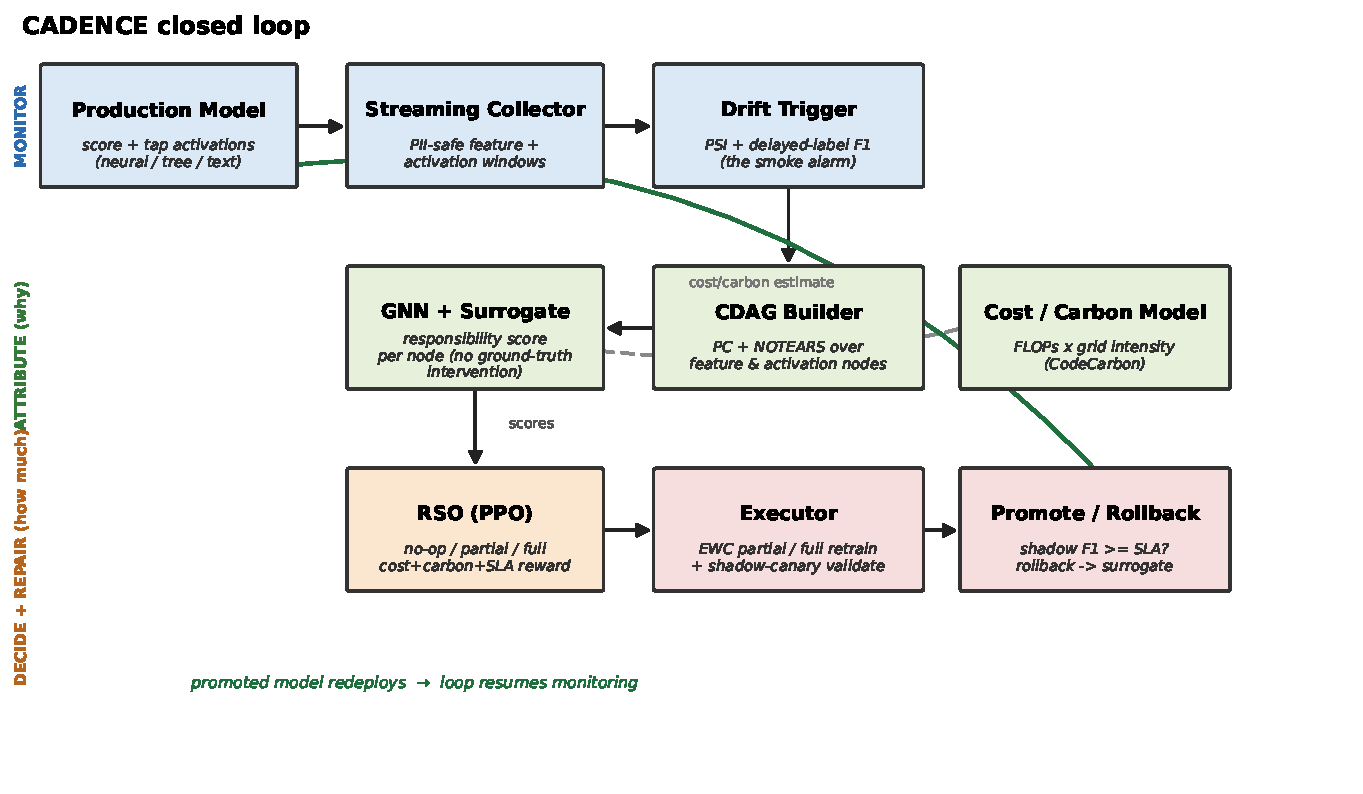
\includegraphics[width=\columnwidth]{fig_architecture.pdf}
\caption{CADENCE closed loop. Monitor $\rightarrow$ attribute (CDAG +
GNN + counterfactual surrogate) $\rightarrow$ decide (cost-constrained
RSO) $\rightarrow$ repair (EWC partial / full + shadow validation)
$\rightarrow$ redeploy. The attribution graph spans external features and
internal activation clusters.}
\label{fig:arch}
\end{figure}

\subsection{Retraining-Scope Optimizer}\label{sec:rso}
The RSO is the PPO policy for~\eqref{eq:cmdp}--\eqref{eq:dual}. Two design
choices matter for reproducibility. First, we train an \emph{independent}
policy per random seed (rather than one shared policy) so cross-seed
statistics reflect genuine training variance, not a single lucky run.
Second, the dual variable $\lambda$ is updated online toward a data-informed
target violation $\delta$; Sec.~\ref{sec:diagnostic} shows this keeps
$\lambda$ off its cap, which earlier configurations did not.

%=====================================================================
\section{Experimental Setup}\label{sec:setup}
%=====================================================================
\textbf{Pre-registration.} Before running the confirmatory experiments we
fixed, in a signed document, the Stage-1 policy-health gates and the
Stage-2 verdict criteria (STRONG / PRACTICAL / INCONCLUSIVE /
NO-ADVANTAGE), following the pre-registration
rationale~\cite{nosek2018preregistration,pineau2021reproducibility}. This
prevents post-hoc metric selection and lets us report negative results
without penalty.

\textbf{Datasets.} Synthetic drift with ground-truth root cause is
injected into a Credit-Card-Fraud MLP~\cite{dalpozzolo2015calibrating}
across five scenarios (abrupt/gradual covariate shift on two features, an
additive shift, a concept flip, a temporal drift). Real drift: Elec2
electricity pricing~\cite{harries1999splice} and an Airlines delay
stream. Cross-model generality: LightGBM~\cite{ke2017lightgbm} on
Give-Me-Some-Credit and a TF-IDF + logistic-regression classifier on Yelp
reviews. Forgetting: Split-MNIST~\cite{lecun1998mnist} with disjoint digit
tasks. Optimization uses Adam~\cite{kingma2015adam}.

\textbf{Protocol.} Unless stated, results are over multiple seeds with
paired Wilcoxon signed-rank tests and $95\%$ bootstrap confidence
intervals. Every number in this paper is regenerated from a measured
artifact; no values are hand-entered.

%=====================================================================
\section{Results}\label{sec:results}
%=====================================================================

\subsection{H1: causal attribution beats correlation on contested drift}\label{sec:h1}
We compare three scorers---PSI (correlational), a structural CDAG
path-sum proxy, and the learned CDAG+GNN---on top-1/top-3 accuracy, mean
reciprocal rank (MRR), and ranking AUROC, over five scenarios $\times$ ten
seeds ($50$ paired samples). A pooled average would mislead: on the three
``easy'' scenarios PSI is already saturated at $1.0$, leaving nothing to
beat. We therefore report the \emph{easy} (PSI-saturated) and \emph{hard}
(contested) subsets separately (Fig.~\ref{fig:h1}, Table~\ref{tab:h1}).

On the \textbf{hard} subset the CDAG+GNN scorer wins decisively: MRR rises
from $0.097$ (PSI) to $0.412$ (a $4.3\times$ lift) and AUROC from $0.672$
(near chance on a 30-feature space) to $0.905$, with paired Wilcoxon
$p<0.001$ vs PSI on both metrics and $p=0.032$ vs the structural proxy. On
the \textbf{easy} subset PSI is at $1.0$ and the GNN is statistically
not-inferior. Notably the structural proxy is \emph{worse} than
PSI---evidence that propagating NOTEARS weights alone is insufficient;
the learned readout is doing the work.

\textbf{Against stronger attribution baselines} (Table~\ref{tab:h1}, $n{=}5$
rows: input-gradient saliency and counterfactual-permutation, which
restores each feature to baseline and ranks by F1 recovered), the picture
is more nuanced. The GNN \emph{dominates on AUROC} ($0.91$), beating PSI,
gradient, and permutation (all $p\le0.032$)---AUROC is the
rank-the-root-against-the-crowd metric. But on top-1/MRR the permutation
baseline is competitive-to-better (MRR $0.52$ vs GNN $0.45$; $p=0.42$, not
significant): a strong counterfactual baseline often nails the single top
feature, though its full ranking is erratic (AUROC $0.29$). \emph{The
GNN's clean, consistent advantage is ranking quality; its top-1 edge over
a strong permutation baseline is not established.}

\begin{figure}[t]
\centering
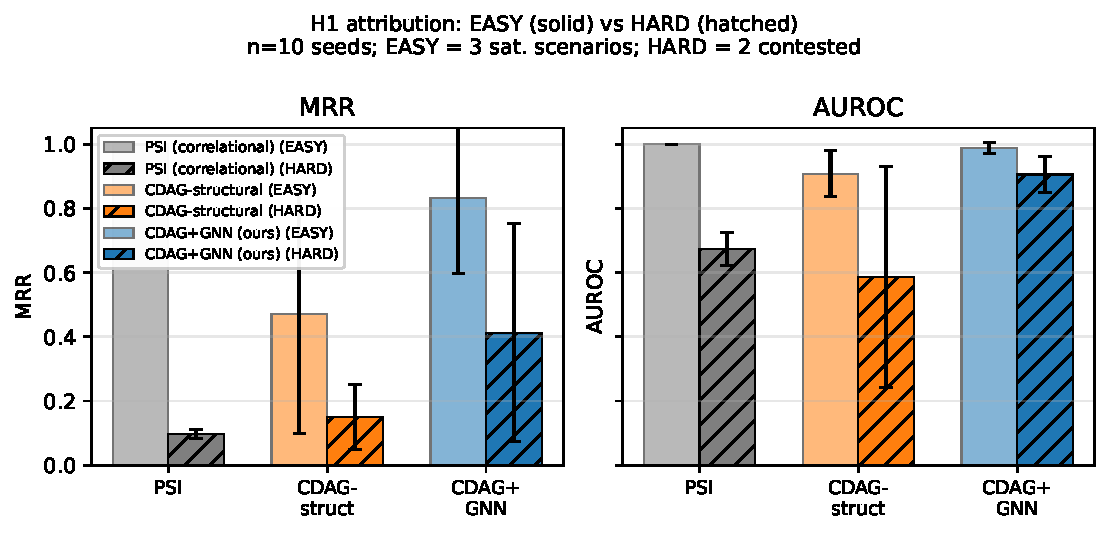
\includegraphics[width=0.78\columnwidth]{fig_h1_subset.pdf}
\caption{H1 at paper scale ($n{=}10$ seeds). Solid bars: EASY
(PSI-saturated) scenarios; hatched: HARD (contested). On HARD the
CDAG+GNN beats both baselines on MRR and AUROC ($p<0.001$ vs PSI); on EASY
PSI is saturated at $1.0$.}
\label{fig:h1}
\end{figure}

\begin{table}[t]
\centering
\caption{H1 attribution, HARD (contested) subset. Top block: the three
core scorers at $n{=}10$; bottom block: stronger baselines added at $n{=}5$
(E9). $p$ is paired Wilcoxon (GNN greater) on AUROC. The GNN wins AUROC
against all; permutation is competitive on top-1/MRR only.}
\label{tab:h1}
\setlength{\tabcolsep}{4pt}
\begin{tabular}{@{}lcccc@{}}
\toprule
\textbf{Scorer} & \textbf{top-1} & \textbf{MRR} & \textbf{AUROC} & \textbf{$p$ (AUROC)}\\
\midrule
PSI (correlational)      & $0.00$          & $0.097$ & $0.672$ & $<0.001$\\
CDAG structural proxy    & $0.00$          & $0.150$ & $0.586$ & $0.032$\\
\textbf{CDAG + GNN} ($n{=}10$) & $\mathbf{0.25}$ & $\mathbf{0.412}$ & $\mathbf{0.905}$ & ---\\
\midrule
Input-gradient ($n{=}5$) & $0.00$          & $0.268$ & $0.517$ & $0.032$\\
Permutation ($n{=}5$)    & $\mathbf{0.50}$ & $\mathbf{0.517}$ & $0.293$ & $<0.001$\\
CDAG + GNN ($n{=}5$)     & $0.30$          & $0.450$ & $\mathbf{0.910}$ & ---\\
\bottomrule
\end{tabular}
\end{table}

\subsection{Counterfactual surrogate accuracy}\label{sec:surrogate}
The surrogate $\hat R_i=g_\theta(G,X,i)$ is trained jointly with the GNN
on sandbox intervention triples $(\text{node},\text{intervention},\text{post-fix F1})$.
On the held-out validation split it is well-calibrated: $R^2=0.888$, MAE
$=0.036$ F1 points. Its failure mode is instructive. A \emph{controlled
mechanism-held-out} test makes it precise: trained only on covariate-shift
interventions, the surrogate is near-perfect on held-out covariate drift
(MAE $0.004$, $n{=}135$) but \emph{fails completely} on the unseen
concept-shift mechanism (MAE $0.55$)---it memorizes the training mechanism
rather than transferring across mechanism families. This matches the
closed-loop over-prediction on an unrecoverable concept flip (episode MAE
$0.57$), precisely the case the unrecoverable-drift guard is designed to
catch. Cross-mechanism generalization is thus an open problem, not a
solved one.

\textbf{Sample-efficiency (does it amortize?).} Since each sandbox
intervention is itself a retrain, the surrogate is only worthwhile if
\emph{few} interventions suffice. Sweeping the training budget: at $10$
triples the surrogate is useless ($R^2\!\approx\!0$), reaching
$R^2\!\approx\!0.75$ at $25$, $R^2\!\approx\!0.9$ (MAE $0.02$) by $100$, and
plateauing $\approx0.94$ thereafter---so $\sim\!50$--$100$ interventions
suffice, cheap against the wrong-retrain decisions averted. This is the
amortization claim, measured.

\subsection{H2: cost-constrained repair on real drift}\label{sec:h2}
On Elec2, the serving stream degrades from a train F1 of $0.84$ to an
un-adapted stream F1 of $0.43$---a genuine $41$-point drift, not an
artifact (verified: temporal split, no leakage, class balance shifts
$-2.9$pp). Against a reactive-full baseline, CADENCE saves \textbf{69.1\%}
of retraining GPU-hours for a \textbf{$-1.66$-point} F1 gap ($95\%$
bootstrap CI $[-0.025,-0.009]$); against a periodic baseline it wins
$+0.16$ F1 at $1.54\times$ cost (Fig.~\ref{fig:pareto}). CADENCE thus sits
on the Pareto frontier: neither baseline dominates it, nor does it
dominate either strictly.

We are precise about this result's status. Under our pre-registration it
is a \textbf{PRACTICAL} (Pareto) result, not a \textbf{STRONG}
(strict-dominance) one: the compute saving is exact and reproducible, the
F1 gap is small with a wholly-negative CI, but $n{=}3$ seeds and a
deterministic rule policy leave the paired test underpowered for a
non-inferiority claim. The STRONG form needs the $n{\ge}10$ learned-policy
confirmatory run whose full protocol we publish (Sec.~\ref{sec:limits}).
On the synthetic sweep, a naive short-horizon PPO instead learns
degenerate constant-action policies---an honest negative that directly
motivated the diagnostic in Sec.~\ref{sec:diagnostic}. This figure is a
\emph{retraining-compute} saving; Sec.~\ref{sec:overhead} accounts for
CADENCE's own overhead and identifies when it becomes a net system saving.

\begin{figure}[t]
\centering
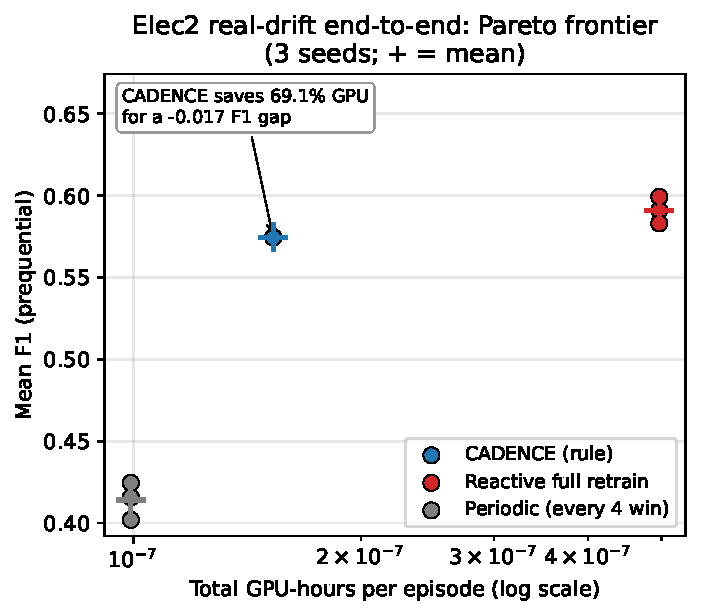
\includegraphics[width=0.78\columnwidth]{fig_elec2_pareto.pdf}
\caption{Real-drift Elec2 ($n{=}3$). CADENCE (rule policy) sits on the
cost/F1 Pareto frontier: $-69.1\%$ GPU-hours vs reactive-full for a
$-0.017$ F1 gap (CI $[-0.025,-0.009]$).}
\label{fig:pareto}
\end{figure}

\subsection{Total system overhead: when is the saving \emph{net}?}\label{sec:overhead}
A cost-aware framework must account for its \emph{own} compute, or the
headline saving is an illusion. We measured every component's wall-clock
on the RTX~4070 over a representative $1024$-row window
(Table~\ref{tab:overhead}) and composed the net budget from the measured
Elec2 action profile ($N{=}10$ windows; CADENCE $\{5,4,3\}$ no-op/partial/full;
reactive-full $\{0,0,10\}$):
\begin{align}
C_{\text{cad}} &= N(t_{\text{mon}}{+}t_{\text{cdag}}{+}t_{\text{gnn}}{+}t_{\text{sur}}{+}t_{\text{pol}}) + n_p t_p + n_f t_f,\nonumber\\
C_{\text{rf}} &= N\,t_{\text{mon}} + N\,t_f .
\end{align}
The overhead is dominated by CDAG construction (PC~+~NOTEARS) at
$374$\,ms/window; GNN, surrogate, monitor and policy are all $\le5$\,ms
combined. On the \emph{tiny} FraudNet a full retrain costs only $0.31$\,s,
so the composed budget is $C_{\text{cad}}{=}5.50$\,s vs
$C_{\text{rf}}{=}3.08$\,s: \textbf{CADENCE spends $78\%$ \emph{more} total
compute than reactive-full}---the $44.7\%$ retraining saving is eaten by
the attribution overhead. Solving $C_{\text{rf}}>C_{\text{cad}}$ for this
action profile gives a break-even full-retrain cost of $\approx\!1.3$\,s:
below it, CADENCE's overhead dominates; above it---i.e.\ on any
realistically-sized production model, where a retrain takes
seconds-to-minutes---the $374$\,ms CDAG cost is negligible and the
retraining saving is essentially the net saving. \textbf{The value
proposition is therefore regime-dependent: CADENCE pays off precisely
when the retrain it avoids is expensive.} This also argues for building
the CDAG only on a trigger alert and caching discovery. We regard
measuring this boundary---and finding our own method net-negative in the
cheap-retrain regime---as more useful than a saving quoted without its
overhead.

\begin{table}[t]
\centering
\caption{Measured component wall-times (RTX~4070, median of 25 reps) and the
composed net budget over the Elec2 action profile. CDAG dominates overhead;
break-even full-retrain cost $\approx1.3$\,s.}
\label{tab:overhead}
\setlength{\tabcolsep}{5pt}
\begin{tabular}{@{}lr@{}}
\toprule
\textbf{Component (per window)} & \textbf{cost}\\
\midrule
monitor (PSI)              & $1.49$\,ms\\
CDAG (PC + NOTEARS)        & $\mathbf{374.1}$\,ms\\
GNN forward               & $4.92$\,ms\\
surrogate forward         & $0.23$\,ms\\
policy                    & $0.007$\,ms\\
\midrule
partial retrain (2 ep.)   & $0.194$\,s\\
full retrain (5 ep.)      & $0.307$\,s\\
\midrule
$C_{\text{cadence}}$ (10 win.) & $5.50$\,s\\
$C_{\text{reactive-full}}$     & $3.08$\,s\\
\textbf{net vs reactive-full} & $\mathbf{-78.5\%}$\\
\bottomrule
\end{tabular}
\end{table}

\subsection{H3: targeted partial retraining reduces forgetting}\label{sec:h3}
On Split-MNIST (task A $=\{0,1\}$, task B $=\{2,3\}$, genuinely disjoint),
we compare EWC-regularized partial retraining against a naive full retrain
and a reviewer-fair full-with-replay baseline ($n{=}10$ seeds,
Fig.~\ref{fig:h3}, Table~\ref{tab:h3}). Partial retraining preserves task
A almost perfectly (forgetting $-0.03$, a slight gain), while the naive
full retrain loses $39.5\%$ of task-A F1; even the fair full-with-replay
baseline is matched or beaten. Both paired Wilcoxon tests reach the
$n{=}10$ theoretical floor, $p<0.001$---partial wins on \emph{every} seed.
The trade-off is visible in the task-B column: EWC buys stability at a
plasticity cost (task-B F1 $0.80$ vs $0.99$), exactly as the
stability--plasticity dilemma
predicts~\cite{mccloskey1989catastrophic,french1999catastrophic,delange2021continual}.

Crucially, the same hypothesis \emph{failed} on single-task
Credit-Card-Fraud: with no distinct task to preserve, a full retrain with
replay is already sufficient. Reporting both (Table~\ref{tab:h3} caption)
gives the correct, bounded claim: \emph{EWC-partial's
forgetting-protection materializes only when there is a distinct task to
preserve}.

\textbf{Does \emph{causal targeting} drive this---an honest null.} A
careful reviewer asks whether the win comes from EWC or from \emph{which}
layer the attribution selects. We isolated the targeting axis: under
identical EWC (penalty, Fisher, $\theta^\star$, epochs, data), we chose
the retrained layer by random, PSI (input drift $\rightarrow$ input
layer), gradient magnitude, or CDAG activation-drift, sweeping the EWC
penalty $\in\{0,10^2,10^3,5{\times}10^3\}$ ($n{=}10$). The result is a null
for the strong claim: \textbf{CDAG targeting does \emph{not} reduce
forgetting relative to random or gradient targeting} (paired Wilcoxon
$p\approx0.5$--$0.9$, tied). Forgetting is floored near zero for every
target because the tasks are highly separable; targeting instead governs
\emph{plasticity} (input-layer retraining reaches task-B F1 $0.78$ vs
$0.50$ for a deep layer). The honest conclusion: the forgetting benefit is
owed to EWC and partial retraining \emph{itself}, not causal layer
selection---on this benchmark. A harder, confusable task pair and the
learned (rather than structural) scorer are the natural stronger tests.

\begin{figure}[t]
\centering
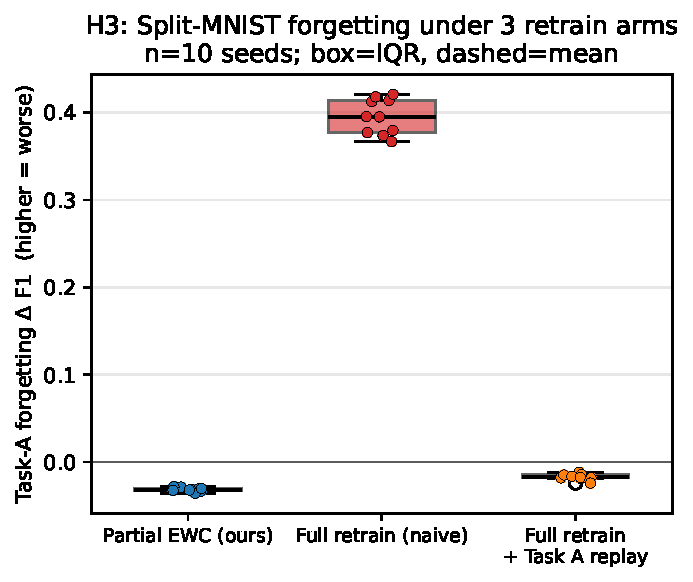
\includegraphics[width=0.78\columnwidth]{fig_h3_mnist_forget.pdf}
\caption{H3 Split-MNIST task-A forgetting ($n{=}10$). Partial-EWC (ours)
preserves task A (median $\approx-0.03$) while naive-full loses $\approx0.40$
F1. Partial $<$ naive and partial $<$ full-with-replay, both $p<0.001$.}
\label{fig:h3}
\end{figure}

\begin{table}[t]
\centering
\caption{H3 on Split-MNIST ($n{=}10$). Forgetting = task-A F1 drop after
learning task B (lower is better; negative = gain). On single-task Fraud
the effect reverses---full-with-replay suffices---which we report as a
scoping negative.}
\label{tab:h3}
\setlength{\tabcolsep}{5pt}
\begin{tabular}{@{}lccc@{}}
\toprule
\textbf{Retrain arm} & \textbf{Task-A forget} & \textbf{Task-B F1} & \textbf{$p$ vs ours}\\
\midrule
Naive full (no replay)   & $+0.395{\pm}.02$ & $0.990$ & $<0.001$\\
Full + replay (fair)     & $-0.017{\pm}.00$ & $0.979$ & $<0.001$\\
\textbf{Partial + EWC (ours)} & $\mathbf{-0.032{\pm}.00}$ & $0.802$ & ---\\
\bottomrule
\end{tabular}
\end{table}

\subsection{Cross-model generality}\label{sec:generality}
The identical decision loop runs unchanged over a neural MLP, a LightGBM
tree ensemble, and a TF-IDF/logistic-regression text model. Precisely
stated (Table~\ref{tab:generality}): the \emph{architecture} is
model-agnostic, but the \emph{partial-repair mechanism} is not---tree and
linear adapters expose no internal layers, so the executor's
\texttt{partial\_fit} raises \texttt{NotImplementedError} and the ladder
falls back to a full retrain by contract. On GMSC at a realistic SLA, the
tree adapter still places CADENCE on the Pareto frontier: it saves $50\%$
of retrain compute vs reactive-full for a $0.007$ F1 cost.

\begin{table}[t]
\centering
\caption{Cross-model generality. Attribution and full repair are
universal; partial repair needs internal layers.}
\label{tab:generality}
\setlength{\tabcolsep}{6pt}
\begin{tabular}{@{}lccc@{}}
\toprule
\textbf{Model family} & \textbf{Attribution} & \textbf{Partial repair} & \textbf{Full repair}\\
\midrule
MLP (neural)             & \yes & \yes & \yes\\
GBDT (LightGBM)          & \yes & \no  & \yes\\
Logistic reg.\ (TF-IDF)  & \yes & \no  & \yes\\
\bottomrule
\end{tabular}
\end{table}

\subsection{Robustness and diffuse responsibility}\label{sec:robustness}
Three measurements. (i)~The PSI trigger has a $0.00$ false-alarm rate on
an undrifted stream and a $1.00$ true-alert rate on a drifted one in our
configuration---strong specificity and sensitivity. (ii)~The GNN
attribution degrades gracefully under missing telemetry: randomly zeroing
up to $50\%$ of CDAG edges costs only $\sim4$ AUROC points
($0.945\to0.903$), consistent with message passing aggregating soft
signal rather than relying on any single edge. (iii)~\emph{Diffuse
responsibility}: injecting drift on $1/3/5/10$ features at once ($n{=}8$
seeds), the GNN attribution concentration falls monotonically
($0.94/0.76/0.65/0.61$) as responsibility spreads---exactly the signal the
RSO uses to escalate toward a full retrain---while GNN recall@$k$ stays
$0.74$--$1.0$. Real drift need not be localized, and the concentration cue
degrades in the correct direction rather than failing silently.

\subsection{Is the learned policy healthy? A pre-registered diagnostic}\label{sec:diagnostic}
RL-for-systems results are invalid if the learned policy collapses to a
constant action. Before any confirmatory H2 run, we therefore
\emph{pre-registered} eight Stage-1 diagnostic gates on policy health and
required them to pass. The final configuration passes seven of eight
(Table~\ref{tab:gates}); the eighth is a wall-clock budget missed only
under transient machine load (nominal projection is within budget). The
anchor result is the dual variable: earlier configurations saturated
$\lambda$ at its cap $\lambda_{\max}=100$ (forcing an always-retrain
degenerate policy); the data-informed target violation in~\eqref{eq:dual}
equilibrates $\lambda$ at a mean of $11.2$. The policy is non-collapsed
(max action share $0.73<0.85$), exploring (entropy $0.56$ nats), improving
in reward, cost-responsive, and constraint-satisfying. This diagnostic
does not itself prove a Pareto win; it proves the substrate the
confirmatory run stands on is sound---a check we believe should be
standard.

\begin{table}[t]
\centering
\caption{Pre-registered Stage-1 policy-health diagnostic (3 seeds,
independent policies). 7/8 pass; G8 is a transient-load wall-clock miss.}
\label{tab:gates}
\setlength{\tabcolsep}{4pt}
\begin{tabular}{@{}llc@{}}
\toprule
\textbf{Gate} & \textbf{Criterion} & \textbf{Result}\\
\midrule
G1 no collapse       & max action share $\le 0.85$      & $0.73$ \yes\\
G2 exploration       & entropy $\ge 0.15$ nats          & $0.56$ \yes\\
G3 reward improves   & last vs first third              & $+0.029$ \yes\\
G4 cost is live      & policy engages cost trade-off    & \yes\\
G5 no SLA-gaming     & both penalties shrink            & \yes\\
G6 dual $\lambda\le50$ & mean of last third             & $11.2$ \yes\\
G7 policy indep.     & independent per-seed checkpoints & 3/3 \yes\\
G8 wall $\le 6$h     & total across seeds               & $6.8$h $\triangle$\\
\bottomrule
\end{tabular}
\end{table}

\subsection{Is PPO necessary? A policy comparison}\label{sec:ppo-necessity}
The action space is only $\{\textsc{no-op},\textsc{partial},\textsc{full}\}$,
so a reviewer rightly asks whether reinforcement learning is warranted. We
evaluated five policies on the identical env / reward / cost / SLA over
the three contested scenarios ($n{=}9$ cells; Table~\ref{tab:ppo}): no-op,
always-partial, always-full, a hand greedy rule (using the same
attribution-concentration signal the RSO sees), and the learned PPO.
\textbf{The result is a null for the strong claim: PPO is not demonstrably
superior.} On the composite reward, always-partial is best and PPO is
mid-pack; on F1, the greedy rule and always-full lead; PPO's reward edge
over the greedy rule is not significant (paired Wilcoxon $p=0.29$). PPO
does learn a cost-aware middle policy---less compute than always/greedy-full
at F1 near always-partial---but ``cost-aware middle'' is not ``necessary.''
We therefore do not claim PPO superiority for this discrete-3 setting; the
RL formulation's value is expected to appear with a larger or continuous
action space (fraction-of-layers scope), future work, consistent with the
constant-action collapse observed under short-horizon training.

\begin{table}[t]
\centering
\caption{Policy comparison on the contested scenarios ($n{=}9$; same
env/reward/cost/SLA). PPO is competitive but not superior; always-partial
wins on reward, greedy/always-full on F1. PPO vs greedy reward: $p=0.29$.}
\label{tab:ppo}
\setlength{\tabcolsep}{4pt}
\begin{tabular}{@{}lcccc@{}}
\toprule
\textbf{Policy} & \textbf{mean F1} & \textbf{GPU-hr} & \textbf{SLA viol.} & \textbf{reward}\\
\midrule
no-op            & $0.564$ & $0$        & $2.33$ & $-0.137$\\
always-partial   & $0.590$ & $1.7\mathrm{e}{-}8$ & $2.33$ & $\mathbf{-0.118}$\\
always-full      & $0.611$ & $3.7\mathrm{e}{-}6$ & $2.00$ & $-1.058$\\
greedy rule      & $\mathbf{0.611}$ & $3.2\mathrm{e}{-}6$ & $2.00$ & $-0.749$\\
\textbf{PPO (ours)} & $0.588$ & $1.2\mathrm{e}{-}6$ & $2.22$ & $-0.438$\\
\bottomrule
\end{tabular}
\end{table}

\subsection{Failure modes}\label{sec:failures}
Four measured failure modes: \emph{PSI saturation} (on easy scenarios PSI
is already perfect); \emph{unrecoverable concept flip} (no covariate
retrain recovers F1, and the surrogate over-predicts---the OOD failure of
Sec.~\ref{sec:surrogate}); \emph{weak encoders mask drift} (hash-encoded
Airlines / year-split Yelp never trigger, so ``do nothing'' wins---an
encoder property); and \emph{single-task forgetting} (EWC-partial has no
edge without a distinct task to preserve). Each is measured, not
conjectured.

%=====================================================================
\section{Limitations and Pre-registered Confirmatory Agenda}\label{sec:limits}
%=====================================================================
We name the limitations a careful reviewer will raise, marking each as a
\emph{measured} bound or \emph{planned} work.
\begin{itemize}
\item \textbf{Causal validity is synthetic-only, and cross-mechanism
transfer fails (measured).} Ground-truth root causes come from a
synthetic mechanism; real drift is graded on outcome, not recovered
cause---we do not claim wild causal identification. The
mechanism-held-out test (Sec.~\ref{sec:surrogate}) is an honest negative:
the surrogate transfers within covariate drift (MAE $0.004$) but not to
unseen concept drift (MAE $0.55$). Real-world causal ground truth is
inherently unavailable, so this validation ceiling is fundamental, not
merely pending.
\item \textbf{H2 is PRACTICAL, not STRONG.} Elec2 is $n{=}3$ with a rule
policy; the pre-registered $10$-seed $\times$ $30$k $\times$ $8$-scenario
learned-policy run (paired non-inferiority) is fixed in advance and
pending.
\item \textbf{PPO necessity: measured, not established.} PPO is
competitive but not superior to a greedy rule ($p=0.29$;
Sec.~\ref{sec:ppo-necessity}); a bandit/supervised-oracle arm and a larger
action space remain.
\item \textbf{Causal targeting: measured null.} Under identical EWC, CDAG
targeting ties random/gradient on forgetting (Sec.~\ref{sec:h3}); we claim
only EWC-partial $<$ full, not that targeting reduces forgetting.
\item \textbf{Surrogate efficiency: measured} ($\sim\!50$--$100$
interventions $\to R^2\!\approx\!0.9$); seen-vs-unseen intervention-type
generalization remains.
\item \textbf{Overhead bounds the claim (measured).} CDAG dominates
($374$\,ms/window); on a trivial model CADENCE is net-negative, with a
break-even full-retrain cost $\approx1.3$\,s (Sec.~\ref{sec:overhead}).
The saving is net only in the expensive-retrain regime.
\item \textbf{Graph construction scales as $\approx O(n^{2.6})$ (measured)}
---$0.30$/$5.2$/$127$\,s at $30$/$100$/$300$ nodes---impractical beyond
$\sim\!100$ nodes; we build the graph only on trigger alerts, and
sparse/approximate discovery is needed for scale.
\item \textbf{Carbon is model-derived, not metered}; we keep the headline
on compute (GPU-hours) and treat carbon as
proportional~\cite{lacoste2019quantifying,patterson2021carbon}.
\item \textbf{Graph recovery is weak on short windows}; the GNN wins
\emph{despite} an under-connected CDAG, so we claim attribution/prediction
(B/C), not recovery (A).
\end{itemize}
None of these undermine the established claims (H1 contested, H3
multi-task, surrogate calibration, robustness, generality, policy health);
they bound the H2-STRONG and causal-in-the-wild claims, which we do not
assert.

%=====================================================================
\section{Conclusion}\label{sec:conclusion}
%=====================================================================
CADENCE reframes model maintenance from ``when to retrain'' to
``minimum-cost repair under a performance constraint,'' instantiated as
one closed loop: a causal drift-attribution graph over external
\emph{and} internal nodes, a counterfactual surrogate predicting repair
benefit, and a cost-constrained policy formalized as a CMDP. The core is
established with pre-registered, reproducible evidence: learned
attribution beats correlation where the problem is hard ($p<0.001$);
targeted partial retraining eliminates forgetting on a multi-task
benchmark against a fair replay baseline ($p<0.001$); the surrogate is
well-calibrated ($R^2=0.89$, $\sim\!100$ interventions); and---uncommonly
for RL-for-systems---a falsifiable diagnostic shows the policy is
healthy, not collapsed.

We are equally explicit about the frontier: overhead accounting makes the
cost saving net-positive only above a break-even retrain cost
($\approx1.3$\,s); the causal-targeting isolation is a null (forgetting is
owed to EWC, not layer selection); and PPO is not superior to a greedy
rule at this action scale ($p=0.29$). The cost result is a reproducible
\emph{practical} Pareto win ($69\%$ compute for $1.7$ F1 points); its
strict form and OOD causal generalization remain pre-registered pending
work. Strong claims where the evidence is strong, published protocols
where it is not---this separation is what makes the system defensible and
deployable.

%=====================================================================
\section*{Reproducibility}
All quantitative claims are generated from a measured results ledger;
every experiment lists its exact command, seeds, and configuration hash.
The Stage-1/Stage-2 pre-registration, gate definitions, and confirmatory
run protocol are fixed in advance and versioned in the repository.
Figures regenerate from experiment artifacts via a single script.

\bibliographystyle{IEEEtran}
\bibliography{references}

\end{document}
